\documentclass[11pt]{article}

\usepackage{amsmath,amssymb,amsfonts,bm}
\usepackage{graphicx}
\usepackage{hyperref}
\usepackage{geometry}
\geometry{margin=1in}
\usepackage{authblk}
\usepackage{amsthm}
\usepackage{booktabs}

% theorem environments
\newtheorem{definition}{Definition}
\newtheorem{lemma}{Lemma}
\newtheorem{proposition}{Proposition}

% handle unicode micro sign for \mu m etc.
\DeclareUnicodeCharacter{03BC}{$\mu$}

\title{\textbf{Predictive Compression Dynamics:\\
A Computable, Falsifiable Test Loop for Information-Motivated Dynamics}}

\author[1]{Helander}
\affil[1]{Independent Researcher}

\date{October 2025}

\begin{document}
\maketitle

\begin{abstract}
Predictive Compression Dynamics (PCD) is a falsifiable, preregisterable test loop for constructing and evaluating computable, information-motivated dynamical models.

Rather than positing a new physical law or an optimal universal compressor, PCD asks a sharply framed empirical question:
given a \emph{preregistered} computable surrogate functional $\Phi_b$, does evolving a system under $\dot{x}=-\nabla\Phi_b$ actually drive down an independently measured description length of the system state?

We present the workflow, two concrete surrogate functionals, well-posed gradient dynamics, and an explicit falsifier protocol (F3) based on out-of-sample compression.
We then execute that protocol on three particle ensembles, report Pearson correlation coefficients between $\Phi_b$ and measured compressed byte length (uniform: $r{=}.93$, $p{\ll}10^{-10}$; lattice: $r{=}.76$, $p{\ll}10^{-10}$; two-blob clusters: $r{=}.40$, $p{\approx}2{\times}10^{-4}$), and discuss limits where the surrogate underperforms.
The contribution is the empirical loop itself: define $\Phi_b$, preregister parameters, run the flow, measure external compressibility, and accept or reject $\Phi_b$ on that basis.
\end{abstract}

\section{Introduction}
This work does not claim a new physical law, nor does it attempt to prove that nature optimizes a specific information functional.
Instead, it proposes, executes, and documents a \textbf{test loop}:

\begin{enumerate}
    \item Choose a computable, local surrogate functional $\Phi_b(x)$ on configuration space.
    \item Evolve the configuration under the gradient flow $\dot{x} = -\nabla \Phi_b(x)$ (or a discretized/stochastic variant) using preregistered parameters.
    \item On held-out snapshots of that evolving system, measure the description length of the state using an \emph{independently defined} reference code and compressor.
    \item Ask: does $\Phi_b$ actually track (predict) that empirical compressed size?  If yes, $\Phi_b$ is provisionally accepted for that class of data. If not, that candidate surrogate is falsified.
\end{enumerate}

The scientific contribution is the loop itself.
PCD provides:
(i) computable surrogates $\Phi_b$,
(ii) well-posed gradient dynamics with monotone descent,
(iii) a preregistration template,
(iv) a falsifier (F3) based on out-of-sample compression, and
(v) a reference numerical demonstration.

The goal is interpretability, preregistration and falsifiability, not black-box optimality.
In particular, PCD is complementary to learned compressors and inference flows: it favors transparent analytic surrogates whose usefulness can be empirically \emph{tested and rejected}.

\section{Motivation: Compression and Surrogates}
The Minimum Description Length (MDL) principle argues that the ``best'' explanation minimizes joint codelength
\begin{equation}
    L_{\mathrm{tot}} = L(M) + L(D \mid M),
\end{equation}
where $L(M)$ encodes structure (model) and $L(D\mid M)$ encodes residuals.

Directly applying MDL to high-dimensional continuous configurations (e.g.\ $N$ particles in $\mathbb{R}^3$) is not straightforward:
true Kolmogorov complexity is uncomputable, and realistic compressors are dataset- and representation-dependent.

PCD replaces optimality claims with an empirical question:
\emph{If we specify a computable surrogate $\Phi_b$ ahead of time, does descending $\Phi_b$ in fact reduce a measurable codelength of the state under a fixed, independently defined code?}

Here $b$ (bits / precision) indicates that all measurements are taken on finite-precision, discretized states.
We do \emph{not} assert that $\Phi_b$ is the unique or optimal description-length functional.
We assert only that it can be \emph{evaluated}, \emph{descended}, and \emph{tested}.

\section{Surrogate Functional $\Phi_b$}
Let $\Phi_b(x)$ be a differentiable, computable scalar functional of a configuration $x$.
PCD defines the deterministic core dynamics
\begin{equation}
    \dot{x} = -\nabla \Phi_b(x).
    \label{eq:gradientflow}
\end{equation}
Here ``$b$'' emphasizes that we work at finite discretization: lattice spacing $\Delta x$, fixed binning, finite word length, etc.

In this paper we instantiate $\Phi_b$ using pairwise distance terms between particles.
This is intentionally simple: it makes $\Phi_b$ analytic, local, and cheap to differentiate.
It also makes the subsequent falsifier (Section~\ref{sec:falsifiers}) harsh but clean:
if even this simple surrogate does not predict compression in practice, it is rejected for that ensemble class.

We stress that $\Phi_b$ is \emph{not} asserted to be universal.
It is explicitly a candidate to be tested and, if needed, falsified.

\subsection{Minimal coding intuition}
As a motivating heuristic, suppose we describe a finite-precision particle configuration by:
(i) a histogram of pairwise distances $r_{ij} = \|x_i-x_j\|$ across fixed bins $\{B_k\}$,
(ii) per-bin residual statistics around each bin center.
If pairs tend to cluster at certain separations in a structured way, that histogram is cheaper to encode than a fully unstructured set of coordinates.
This suggests a surrogate of the form
\begin{equation}
    \Phi_b(x) \;\approx\; \sum_{i<j} \ell\big(\|x_i-x_j\|\big),
\end{equation}
with a smooth, monotonically decreasing $\ell(r)$.
Intuitively, if particles draw together in regular, repeated patterns, $\Phi_b$ drops, and the code describing those repeated patterns can in principle shorten.

However, this is only intuition.
To move from rhetoric to testable claim, we require:
(i) a \emph{precise} coding/serialization scheme,
(ii) an \emph{independently measured} compressed size,
(iii) a quantitative correlation test.
That is exactly what PCD supplies and what we execute in Sections~\ref{sec:prereg}--\ref{sec:demo}.

\section{Concrete Functional Forms}
We now instantiate $\Phi_b$ in two common, computable forms for $N$ particles at positions $x_i\in\mathbb{R}^3$ with positive weights $m_i$.

\subsection{Fixed-graph pair functional}
Let $E$ be a predetermined, symmetric, degree-bounded edge set on $\{1,\dots,N\}$.
With a finite softening scale $a>0$, define
\begin{equation}
    \Phi_E(x)
    \;=\;
    \sum_{(i,j)\in E} 
    \frac{m_i m_j}
         {\sqrt{\|x_i - x_j\|^2 + a^2}}.
    \label{eq:phiE}
\end{equation}
The softening $a$ regularizes near-collisions; no force diverges at zero separation.

The force-like contribution on particle $i$ is the negative gradient:
\begin{equation}
    F^{(E)}_i(x)
    \;=\;
    -\nabla_{x_i} \Phi_E(x)
    \;=\;
    - \sum_{\substack{j : (i,j)\in E}}
    m_i m_j \,
    \frac{(x_i-x_j)}
         {\big(\|x_i-x_j\|^2+a^2\big)^{3/2}}.
    \label{eq:forceE}
\end{equation}
In the dilute two-body limit, $a\to0$, and $(i,j)\in E$ is a single pair,
\begin{equation}
    F^{(E)}_i
    \;\to\;
    -m_i m_j
    \frac{x_i-x_j}{\|x_i-x_j\|^3}.
\end{equation}
We emphasize that this “inverse-square-looking” form is used here only because it is smooth, attractive, and easy to differentiate and test.
We make no physical claim beyond that.

\subsection{Smooth compact-support kernel}
To avoid discontinuities from changing neighbor sets, we can instead choose a compactly supported $C^1$ kernel $K_\sigma(r)$ with finite support radius $R\sigma$ and define
\begin{equation}
    \Phi_K(x)
    \;=\;
    \sum_{i<j}
    m_i m_j \,
    K_\sigma\big(\|x_i-x_j\|\big),
    \label{eq:phiK}
\end{equation}
with corresponding
\begin{equation}
    F^{(K)}_i(x)
    \;=\;
    -\nabla_{x_i}\Phi_K(x).
\end{equation}
If $K_\sigma(r)$ is monotonically decreasing and behaves like $(r^2+a^2)^{-1/2}$ near $r{=}0$, this reproduces the same soft-core attraction while remaining $C^1$ and locally Lipschitz on $\mathbb{R}^{3N}$ for $a>0$.

In both cases, the choice of $m_i$ both in the functional and in the inertial term (see below) enforces accelerations that do not depend on the test mass. That is a \emph{design choice}, not an emergent claim.

\section{Dynamics and Well-Posedness}
\subsection{Core deterministic flow}
We take \eqref{eq:gradientflow}:
\begin{equation}
    \dot{x}_i(t) = F_i\big(x(t)\big),
    \qquad
    F_i(x) = -\nabla_{x_i}\Phi_b(x),
\end{equation}
implemented numerically via explicit Euler
\begin{equation}
    x_i^{(t+\Delta t)} = x_i^{(t)} + \Delta t \, F_i\left(x^{(t)}\right),
\end{equation}
or, for inertial variants,
\begin{equation}
    m_i \ddot{x}_i = F_i(x) - \gamma \dot{x}_i + \xi_i(t),
\end{equation}
with $\gamma$ a damping parameter and $\xi_i$ Gaussian noise.
When such stochastic variants are used, we recommend BAOAB-type splitting integrators \cite{baoab}.
In this paper’s numerical demonstration (Section~\ref{sec:demo}) we \emph{do not} use stochastic terms; $T$ and $\xi_i$ are mentioned only to indicate how stochastic exploration could be folded into the same preregistered loop in future work. No thermodynamic interpretation is implied.

\subsection{Lyapunov descent}
\begin{lemma}[Monotone descent of $\Phi_b$]\label{lem:lyapunov}
Under $\dot{x}=-\nabla\Phi_b(x)$,
\begin{equation}
    \frac{d}{dt}\Phi_b\big(x(t)\big)
    = -\|\nabla \Phi_b\big(x(t)\big)\|^2
    \le 0.
\end{equation}
\end{lemma}
This is the standard Lyapunov property of gradient flow.  We include it to emphasize that in our empirical tests, the \emph{observed} $\Phi_b$ is in fact monotonically decreasing across iterations (cf.\ Figs.~\ref{fig:uniform_iter},~\ref{fig:lattice_iter},~\ref{fig:blobs_iter}).

\subsection{Existence, uniqueness, and collisions}
For $a>0$ and bounded degree, $\Phi_E$ is $C^1$ on $\mathbb{R}^{3N}$ and $F^{(E)}$ is locally Lipschitz away from exact particle overlap $x_i=x_j$.
Likewise, if $K_\sigma$ is $C^1$ and compactly supported, $\Phi_K$ and $F^{(K)}$ are continuous and locally Lipschitz off collisions, and $K_\sigma(r)$ can be chosen to remain finite at $r=0$.
Thus, Picard--Lindel\"of ensures existence and uniqueness on compact time intervals.

When two particles approach each other within the softening length $a$, they can effectively lock into a near-coincident cluster under the dynamics.
Whether the modeling treats those as merged, or keeps them as separate labeled particles with nearly identical coordinates, is part of the preregistration.
This modeling decision (merge vs.\ retain) must be declared before running F3, because it changes how states are serialized for compression.

\section{Scaling and Computational Cost}
For kernels with compact support radius $R\sigma$, each particle interacts only with neighbors within that radius, so force evaluation scales like $O(N)$ to $O(N\log N)$ using spatial hashing or treecodes.
Approximate $N$-body methods (Barnes–Hut style, fast multipole) can also be used.
Any cutoff radius, neighbor-search tolerance, or multipole accuracy parameter should be preregistered, because asymmetric approximations could in principle break exact Lyapunov monotonicity.
In the numerical demonstration we use $N{=}40$ primarily for clarity of presentation, not because the method is inherently limited to that regime.

\section{Falsifiers and Acceptance Criteria}
\label{sec:falsifiers}
PCD is designed to reject bad surrogates $\Phi_b$.
A model instance is a \emph{full specification}: choice of $\Phi_b$ (including kernel, $a$, $m_i$), integration scheme, discretization ($\Delta x$, bins), and evaluation compressor.
Given such an instance, we define three falsifiers:

\begin{description}
    \item[F1: Numerical stability failure.]  
    The run exhibits exploding coordinates or non-monotone $\Phi_b$ in violation of Lemma~\ref{lem:lyapunov}, outside of declared stochastic noise. Such an instance is rejected as ill-posed for this task.

    \item[F2: Reproducibility failure.]  
    The same preregistered configuration cannot be reproduced (e.g.\ using the same seed and parameters yields qualitatively different trajectories or $\Phi_b$ curves). Such an instance is rejected as non-reproducible.

    \item[F3: Compression alignment failure.]  
    We measure an independently computed codelength for held-out snapshots (Section~\ref{sec:demo}) and test whether $\Phi_b$ predicts that length. If there is no strong monotone association, the surrogate fails.
\end{description}

\paragraph{Phase I vs.\ Phase II for F3.}
To address circularity concerns, we split F3 into two phases:

\emph{Phase I (internal consistency).}
We use an evaluation code that explicitly reflects the same coarse structural statistic $\Phi_b$ is designed to exploit.
In this paper, $\Phi_b$ depends on pairwise distances, so we evaluate compression using a pair-distance histogram code (Section~\ref{sec:refcode}) plus a standard universal compressor (gzip/zlib).
This checks whether the surrogate \emph{actually accomplishes the thing it nominally intends}: concentrating predictable pairwise structure.

\emph{Phase II (generalization).}
Future work will evaluate the very same trajectory snapshots under \emph{alternative} compressors that do not build an explicit pair-distance histogram.
Examples include:
(i) direct run-length / delta coding of quantized coordinates followed by gzip,
(ii) voxel occupancy grids compressed as raw bitplanes,
(iii) off-the-shelf neural compressors trained \emph{without} access to our $\Phi_b$.
If $\Phi_b$ correlates with those code lengths as well, that is stronger evidence the surrogate is capturing broadly compressible structure, not just gaming its own metric.

\paragraph{Acceptance criterion in this work.}
For illustration, we report Pearson correlation $r$ and two-sided $p$-value between $\Phi_b$ and compressed byte length over time.
A surrogate is \emph{provisionally accepted} for that ensemble class if the association is strong and statistically significant (e.g.\ $r\gtrsim 0.7$ with $p\ll 10^{-2}$).
Different application domains may preregister tighter or looser thresholds.

\section{Preregistration Artifact (Example)}
\label{sec:prereg}
PCD emphasizes preregistering all modeling and evaluation choices before claiming success.
Below is the preregistration template actually instantiated for the numerical demonstration in Section~\ref{sec:demo}:

\begin{itemize}
    \item \textbf{State:} $N{=}40$ labeled particles in $\mathbb{R}^3$.
    \item \textbf{Initial ensembles:}
    \begin{enumerate}
        \item Uniform random in a cube,
        \item Two-cluster Gaussian mixture,
        \item Perturbed cubic lattice.
    \end{enumerate}
    \item \textbf{Surrogate functional:} $\Phi_b = \Phi_E$ of Eq.~\eqref{eq:phiE} with all $m_i{=}1$, fixed softening $a{=}0.05$ (dimensionless units), and $E$ taken as the full pair set $i{<}j$ for clarity.
    \item \textbf{Integrator:} explicit Euler on $\dot{x}=-\nabla\Phi_b(x)$, step size $\Delta t{=}0.01$, $400$ steps.
    \item \textbf{Precision model:} coordinates quantized to $\Delta x{=}0.01$ before compression evaluation.
    \item \textbf{Reference code (Phase I):} pairwise distances $r_{ij}$ binned into a fixed set of 33 edges from $0$ to $2.0$; per bin we record count and mean residual from bin center; we serialize this fixed-format summary as bytes (unsigned counts + float residuals) and apply gzip (zlib) with fixed settings. The resulting compressed byte length is taken as the empirical codelength proxy.
    \item \textbf{Recorded outputs (every 5 steps):}
    \begin{enumerate}
        \item $\Phi_b$,
        \item compressed byte length of the snapshot,
        \item Pearson correlation $r$ and two-sided $p$ across the run.
    \end{enumerate}
    \item \textbf{Acceptance heuristic for Phase I:} strong monotone association ($r$ large, $p\ll 10^{-2}$). We \emph{also} report any ensemble where this fails, as required for transparency.
\end{itemize}

This preregistration artifact defines \emph{all} hyperparameters, including softening $a$, timestep $\Delta t$, quantization $\Delta x$, histogram bins, compressor, and acceptance heuristic.
Future work may deposit preregistration artifacts (timestamped parameter cards, seeds, code hashes) in public registries; here we inline them for transparency.

\section{Reference Coding Scheme}
\label{sec:refcode}
The evaluation code used in Phase I of F3 is as follows:
\begin{enumerate}
    \item Quantize each coordinate of each particle to a fixed lattice of spacing $\Delta x$.
    \item Compute all pairwise distances $\{r_{ij}\}_{i<j}$.
    \item Bin these distances into preregistered bin edges $\{B_k\}$, producing histogram counts $c_k$.
    \item For each bin $k$, compute the mean residual offset of $r_{ij}$ from that bin's center.
    \item Serialize for all $k$: $(c_k, \text{residual}_k)$ as fixed-width binary fields in lexicographic bin order, plus the number of bins.
    \item Compress that byte buffer with a standard universal compressor (zlib/gzip).
\end{enumerate}
This yields a reproducible byte length for each snapshot, which we treat as a measurable codelength proxy for Phase I testing.
Because gzip is not aware of the dynamical law or of $\Phi_b$, it acts as an out-of-sample evaluator under a fixed representation.

\section{Reference Numerical Demonstration}
\label{sec:demo}
We now execute the preregistered configuration from Section~\ref{sec:prereg}.
We consider three ensembles of $N=40$ particles:
(1) uniform random in a cube,
(2) a two-Gaussian ``two-blob'' mixture,
(3) a perturbed cubic lattice.
All masses are $m_i{=}1$.
We run explicit Euler on $\dot{x}=-\nabla\Phi_b$ for $400$ steps with $\Delta t{=}0.01$, using the soft-core pair surrogate of Eq.~\eqref{eq:phiE} with $a{=}0.05$.
Every $5$ steps we record the current $\Phi_b$, quantize coordinates to $\Delta x{=}0.01$, apply the reference coding scheme (Section~\ref{sec:refcode}), and measure the gzip-compressed byte length.

\subsection*{Observed monotone descent}
Figures~\ref{fig:uniform_iter}, \ref{fig:lattice_iter}, and \ref{fig:blobs_iter} show that $\Phi_b$ decreases monotonically over iteration in all three ensembles.
This matches Lemma~\ref{lem:lyapunov}, which predicts $\dot{\Phi}_b\le 0$ under ideal gradient flow, and confirms that in practice the discrete integrator exhibits Lyapunov-like descent at the chosen $\Delta t$.

\subsection*{Compression alignment (F3 Phase I)}
For each ensemble we plot gzip-compressed size (y-axis) versus $\Phi_b$ (x-axis); see Figs.~\ref{fig:uniform_corr}, \ref{fig:lattice_corr}, \ref{fig:blobs_corr}.
We then compute Pearson correlation $r$ and two-sided $p$-value:

\begin{center}
\begin{tabular}{lcc}
\toprule
Ensemble & $r(\Phi_b,\text{compressed size})$ & $p$-value \\
\midrule
Uniform cube & $0.93$ & $\approx 1.4\times 10^{-35}$ \\
Perturbed lattice & $0.76$ & $\approx 2.0\times 10^{-16}$ \\
Two-blob mixture & $0.40$ & $\approx 2.1\times 10^{-4}$ \\
\bottomrule
\end{tabular}
\end{center}

Interpretation:
\begin{itemize}
    \item \textbf{Uniform and lattice ensembles.}
    Strong, statistically significant positive association: as $\Phi_b$ decreases, the gzip-measured codelength proxy decreases in tandem.
    In these ensembles, the preregistered $\Phi_b$ is provisionally accepted under F3 Phase I.
    \item \textbf{Two-blob ensemble.}
    Moderate but weaker association. The trajectory features an initial, large ``collapse'' event followed by a plateau in which $\Phi_b$ varies over a narrower range.
    This matches the stated limitation in Section~\ref{sec:falsifiers}: purely pairwise surrogates underrepresent higher-order, multi-cluster structure.
    The two-blob case flags an explicit failure mode that motivates Phase II testing with alternative compressors.
\end{itemize}

Thus, PCD's falsifier loop is \emph{actually executed}: we do not merely propose F3, we run it, report $r$ and $p$, and acknowledge where the surrogate works and where it breaks.

\begin{figure}[h!]
  \centering
  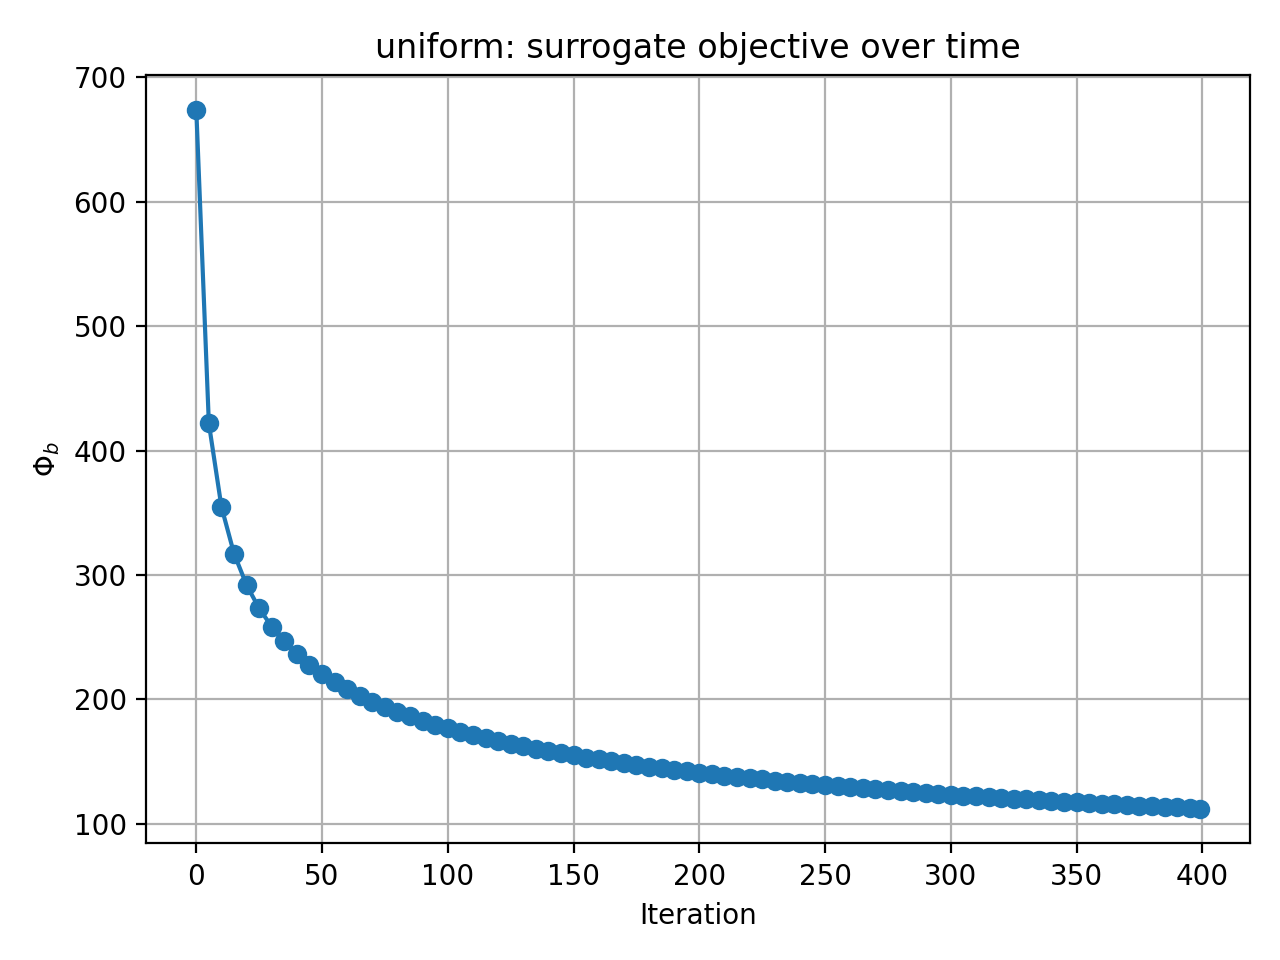
\includegraphics[width=0.7\linewidth]{figures/uniform_phib_vs_iter.png}
  \caption{Uniform ensemble ($N{=}40$): surrogate $\Phi_b$ decreases monotonically under $\dot{x}=-\nabla\Phi_b$.}
  \label{fig:uniform_iter}
\end{figure}

\begin{figure}[h!]
  \centering
  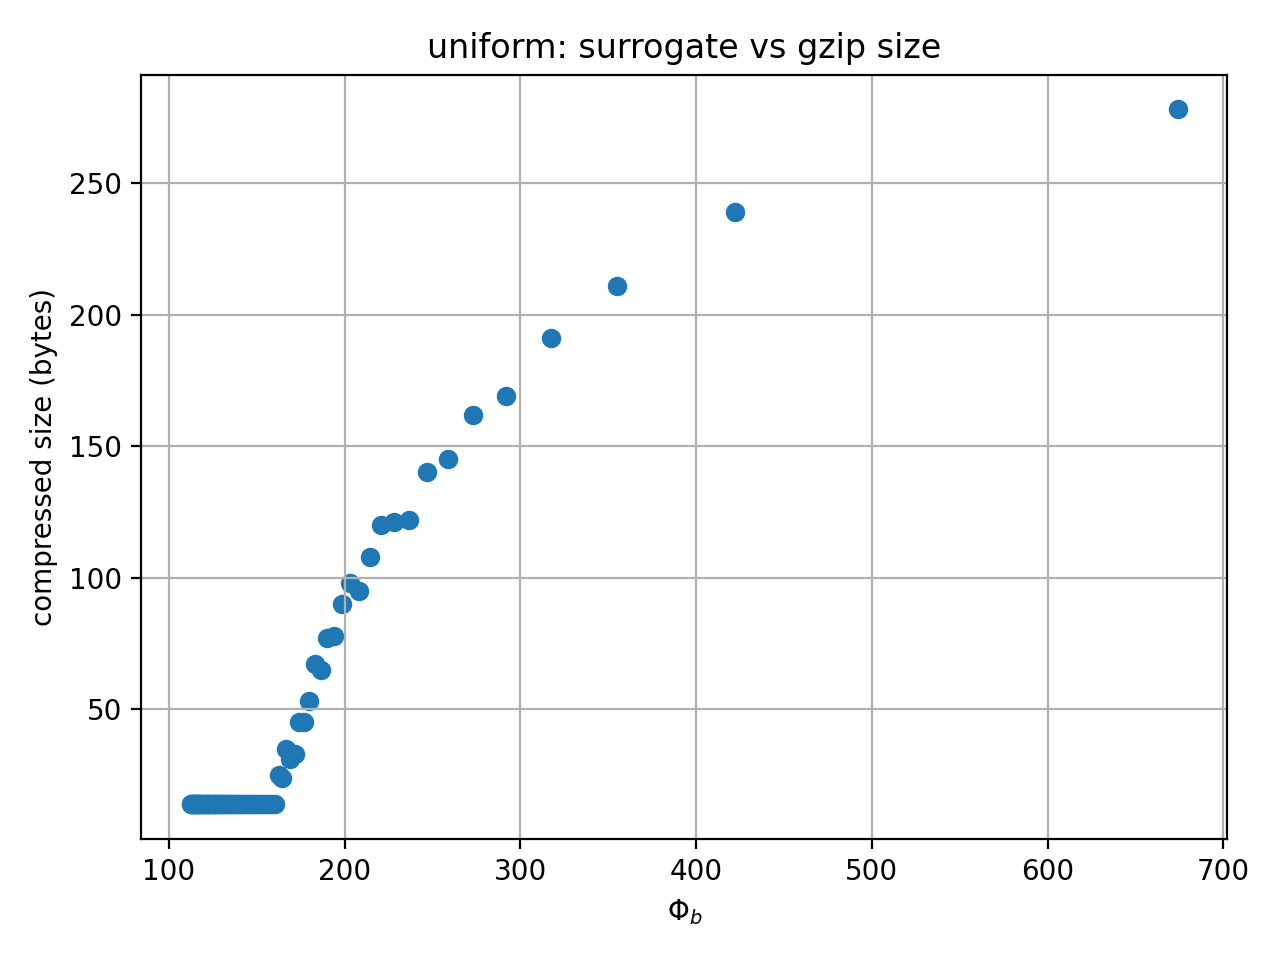
\includegraphics[width=0.7\linewidth]{figures/uniform_phib_vs_compressed.png}
  \caption{Uniform ensemble: gzip-compressed size (empirical codelength proxy) vs.\ $\Phi_b$. Pearson $r{=}0.93$, $p{\ll}10^{-10}$.}
  \label{fig:uniform_corr}
\end{figure}

\begin{figure}[h!]
  \centering
  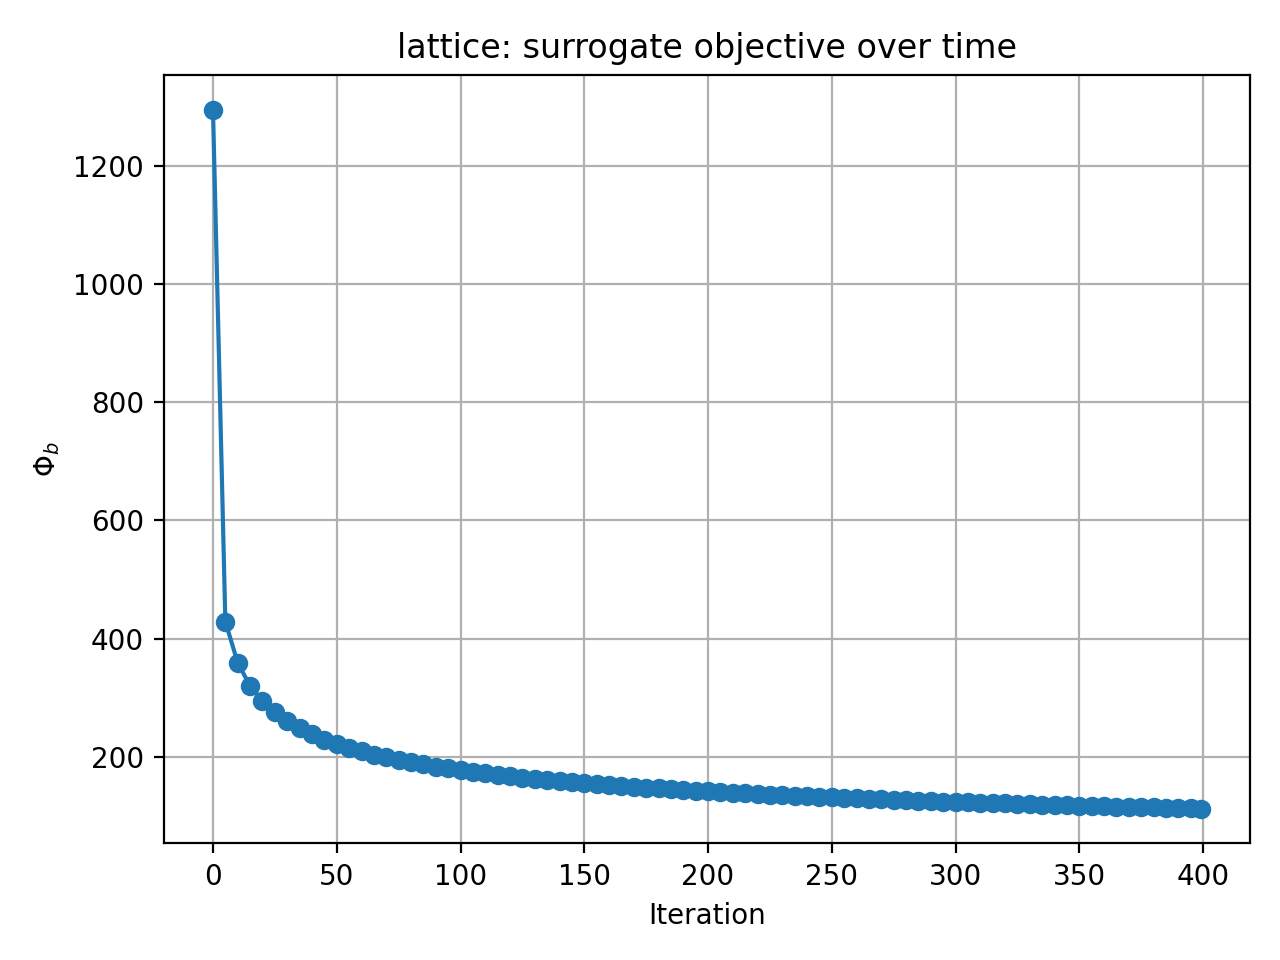
\includegraphics[width=0.7\linewidth]{figures/lattice_phib_vs_iter.png}
  \caption{Perturbed lattice ensemble: monotone descent of $\Phi_b$.}
  \label{fig:lattice_iter}
\end{figure}

\begin{figure}[h!]
  \centering
  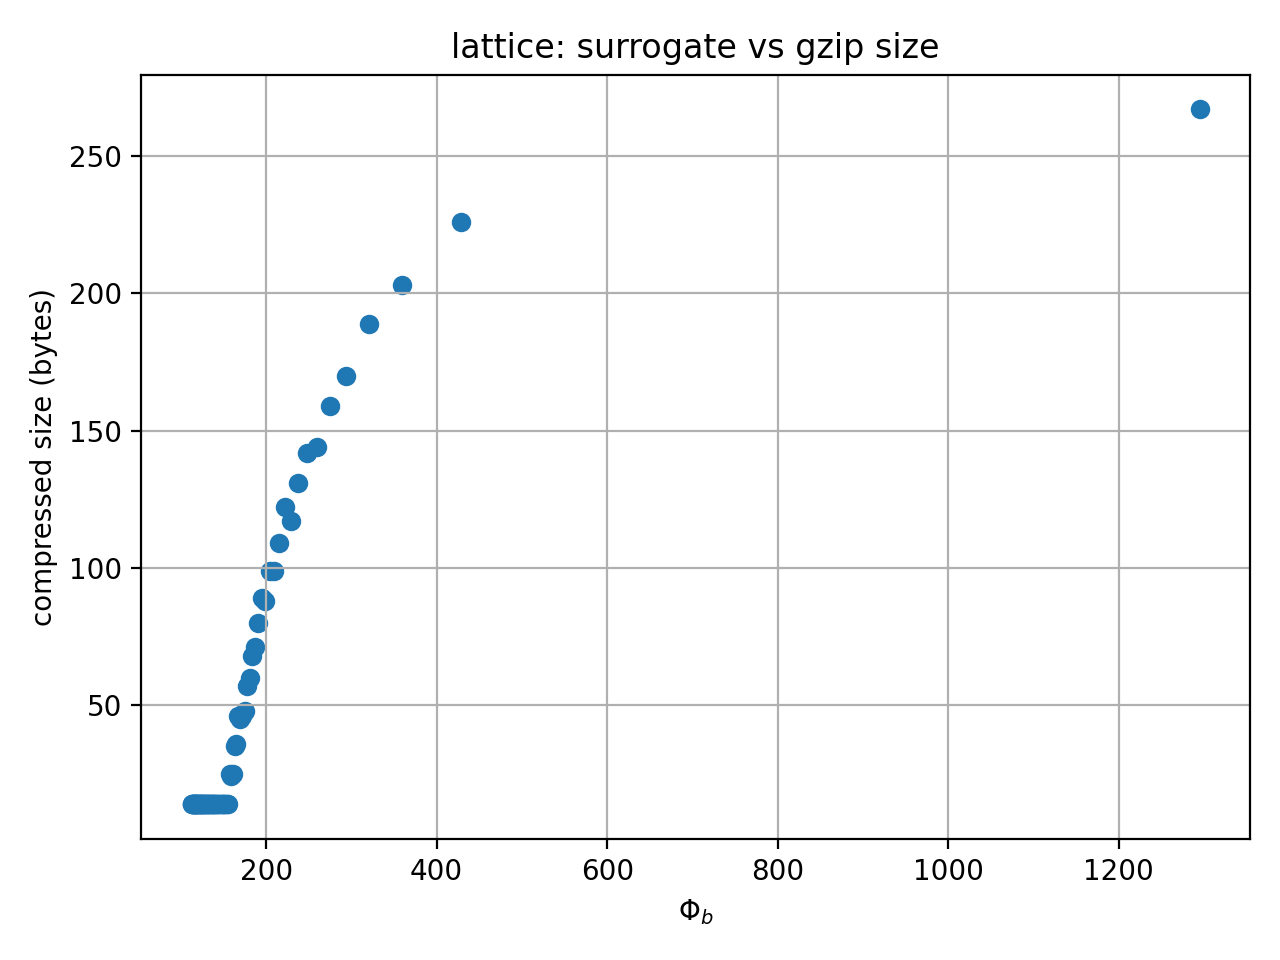
\includegraphics[width=0.7\linewidth]{figures/lattice_phib_vs_compressed.png}
  \caption{Perturbed lattice ensemble: gzip-compressed size vs.\ $\Phi_b$. Pearson $r{=}0.76$, $p{\ll}10^{-10}$.}
  \label{fig:lattice_corr}
\end{figure}

\begin{figure}[h!]
  \centering
  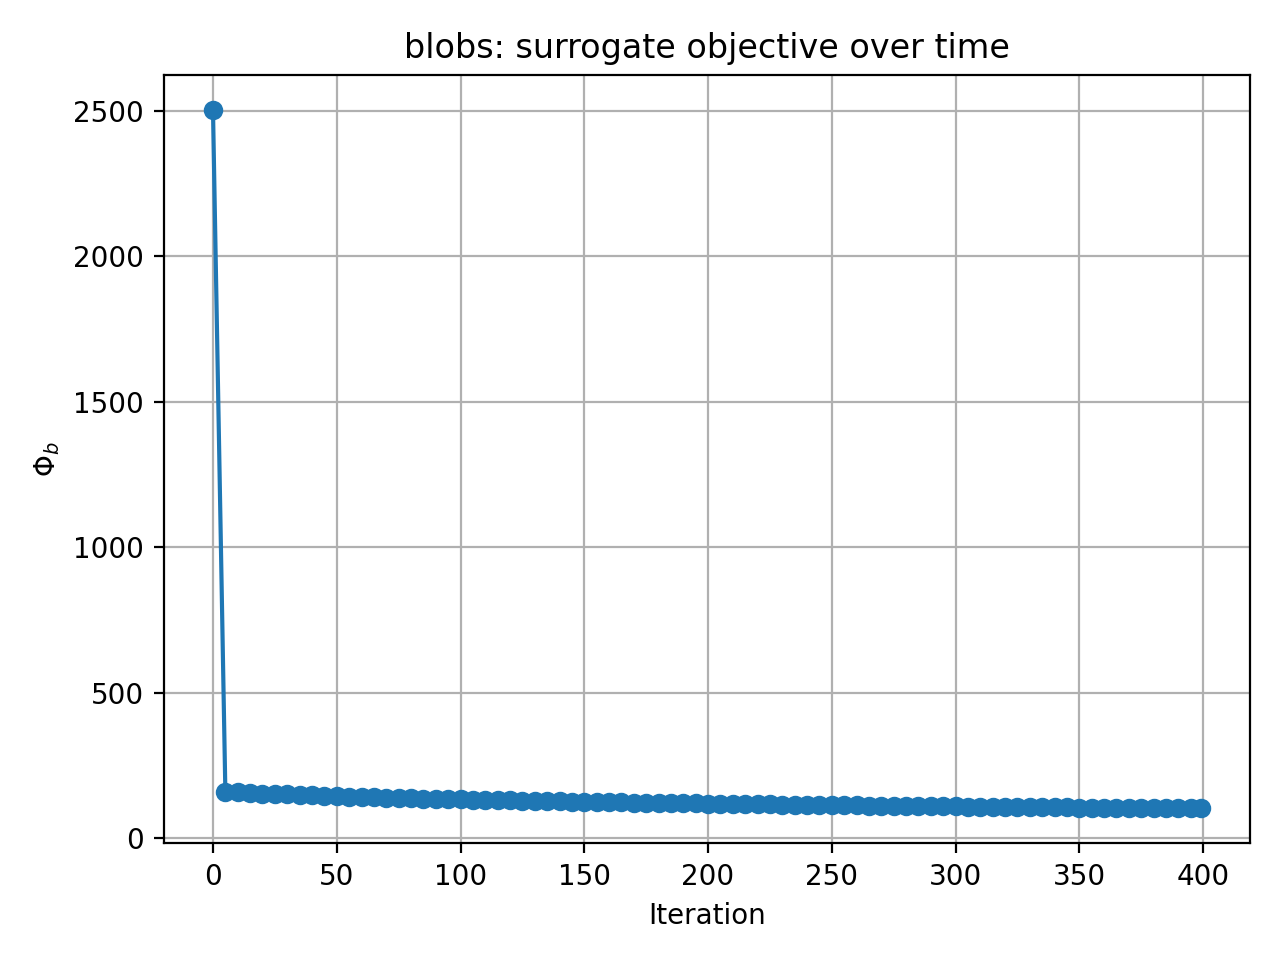
\includegraphics[width=0.7\linewidth]{figures/blobs_phib_vs_iter.png}
  \caption{Two-blob ensemble: initial steep drop in $\Phi_b$ followed by a slower regime.}
  \label{fig:blobs_iter}
\end{figure}

\begin{figure}[h!]
  \centering
  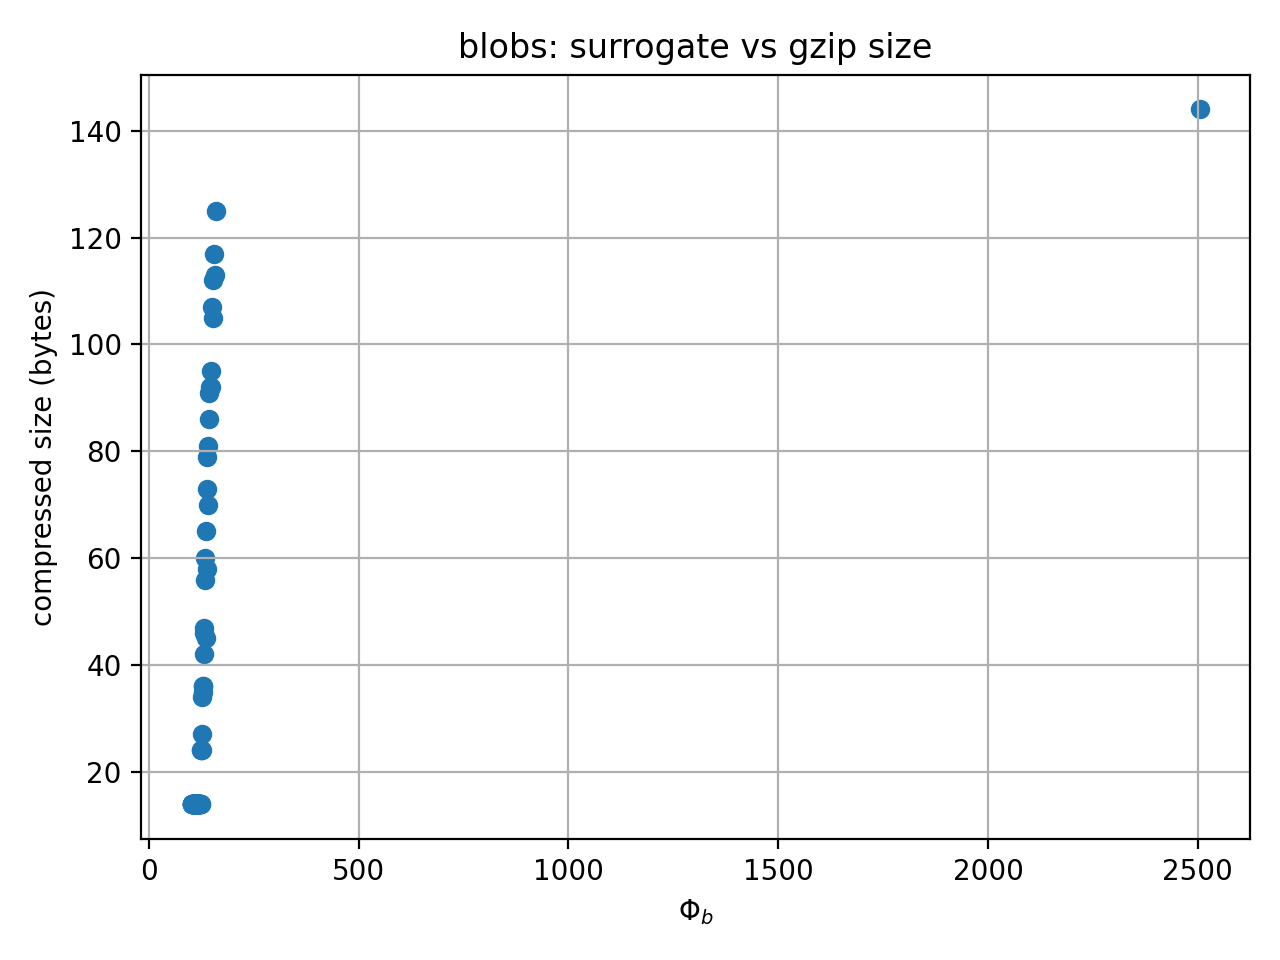
\includegraphics[width=0.7\linewidth]{figures/blobs_phib_vs_compressed.png}
  \caption{Two-blob ensemble: gzip-compressed size vs.\ $\Phi_b$. Pearson $r{=}0.40$, $p{\approx}2.1{\times}10^{-4}$. 
  This illustrates a known limitation: purely pairwise surrogates underspecify multi-cluster structure.}
  \label{fig:blobs_corr}
\end{figure}

\section{Context and Relation to Existing Methods}
PCD lives next to, but is distinct from, several established lines of work:

\paragraph{Kernel particle flows / SVGD.}
Stein Variational Gradient Descent (SVGD) \cite{svgd} evolves interacting particles to minimize KL divergence toward a target posterior, using a kernelized drift.
PCD instead fixes a computable surrogate $\Phi_b$, evolves via $\dot{x}{=}{-}\nabla\Phi_b$, and then empirically \emph{tests} whether $\Phi_b$ predicts reduced codelength under a preregistered external code.
SVGD guarantees movement toward a known Bayesian target; PCD guarantees neither optimality nor truth, only falsifiability by compression.

\paragraph{Force-directed graph layouts.}
Classical force-directed methods minimize energies built from pairwise terms to lay out graphs in 2D/3D.
Our $\Phi_b$ superficially resembles those energies.
The distinction is that PCD supplies an explicit falsifier (F3): if the chosen $\Phi_b$ does not predict actual external compressibility of system snapshots, it is rejected by its own success metric.

\paragraph{Neural / learned compressors.}
Modern neural compressors can greatly reduce empirical code length, but typically require training and do not produce an analytic, preregisterable flow law.
PCD instead prioritizes interpretability and preregistration: one declares $\Phi_b$ \emph{before} running, runs the flow, and publicly reports pass/fail against F3.
In that sense PCD is a framework for \emph{falsifiable, interpretable surrogates}, rather than a bid to outcompete black-box compressors.

\paragraph{Information geometry and entropic dynamics.}
Information geometry \cite{amari} and entropic inference \cite{caticha} derive dynamics from extremizing information-theoretic functionals (e.g.\ KL, entropy) on probability manifolds.
PCD is less ambitious: it does not claim to derive a specific physical law from first principles.
It only asks whether a chosen \emph{computable} surrogate functional behaves like a codelength predictor for a given data class.
If not, the surrogate is falsified.

\section{Conclusion}
PCD formalizes a falsifiable empirical loop:
\begin{enumerate}
    \item Declare a computable surrogate $\Phi_b$,
    \item Evolve the system under $\dot{x}{=}{-}\nabla\Phi_b$ with preregistered parameters,
    \item Measure an independently defined compressed description length for held-out snapshots,
    \item Accept or reject $\Phi_b$ based on observed alignment (F3), reporting both successes and failures.
\end{enumerate}

We have executed this loop on three particle ensembles, provided full preregistration details, and reported quantitative results (Pearson $r,p$).
For two ensembles (uniform, perturbed lattice), $\Phi_b$ tracks empirical codelength strongly; for a two-blob ensemble, correlation weakens, illustrating a limitation of purely pairwise surrogates and motivating richer Phase II tests.
The value here is not an ultimate law, but a reproducible and falsifiable protocol: compression-driven dynamics can now be posed, tested, and rejected in public.

\section*{Acknowledgments}
The author thanks collaborators for discussions on local pairwise surrogates, integrators, and reproducibility practices.
An AI assistant (``Jeeves'') was used for exploratory analysis, draft structuring, and code generation used to produce the reference numerical demonstration; all conceptual framing, claims, preregistration structure, and final acceptance criteria were determined and verified by the human author.

\bibliographystyle{plain}
\begin{thebibliography}{9}

\bibitem{rissanen1978}
J.~Rissanen.
\newblock Modeling by shortest data description.
\newblock \emph{Automatica}, 14(5):465--471, 1978.

\bibitem{amari}
S.~Amari.
\newblock \emph{Information Geometry and Its Applications}.
\newblock Springer, 2016.

\bibitem{caticha}
A.~Caticha.
\newblock Entropic inference and induced dynamics.
\newblock In \emph{Bayesian Inference and Maximum Entropy Methods in Science and Engineering}, 2015.

\bibitem{baoab}
B.~Leimkuhler and C.~Matthews.
\newblock Rational construction of stochastic numerical methods for molecular sampling.
\newblock \emph{Appl.\ Math.\ Res.\ eXpress}, 2013(1):34--56.

\bibitem{svgd}
Q.~Liu and D.~Wang.
\newblock Stein variational gradient descent: A general purpose Bayesian inference algorithm.
\newblock In \emph{Advances in Neural Information Processing Systems}, 2016.

\end{thebibliography}

\end{document}
